\documentclass[letterpaper,12pt,twoside=false,DIV=11]{scrbook}

%----------------------CONFIG---------------------------
%math packages
\usepackage{amsmath,amssymb,amsthm,units,unitsdef}
\usepackage{wasysym}  % astro symbols

%bibliography style and citation style, bibstyles to use: plainnat, abbrvnat, unsrtnat, named, chicago
%otherwise numerical citationstyle will be used
\usepackage[authoryear,round]{natbib}
\usepackage{longtable,tabularx,tabulary,multirow,lscape}
\usepackage[font={sl},format=plain,labelfont=bf]{caption}

% appendix
\usepackage{appendix}
\usepackage{xpatch}
\xpretocmd{\appendixpagename}{\sffamily}{}{}

% colors
\usepackage{color,colortbl}
\usepackage[dvipsnames]{xcolor}
\definecolor{darkblue}{HTML}{00354C}

\usepackage{booktabs}
% \usepackage{showkeys} % shows the labels above the references for

%easier development
\usepackage{ifpdf}

\ifpdf
	\usepackage[pdftex]{graphicx}
	\usepackage[]{pdfpages} %for including full pdf pages
	\usepackage[pdftex,
		bookmarks,
		bookmarksopen=true,
		bookmarksnumbered=true,
		pdfauthor={Reto Trappitsch},
		pdftitle={Introduction Arduino},
		colorlinks,
		linkcolor=darkblue,
		citecolor=darkblue,
		filecolor=black,
		urlcolor=darkblue,
		anchorcolor=black,
		menucolor=black,
		breaklinks=true,
		pageanchor=true, %for jumping to a page
		plainpages=false,
		pdfpagelabels=true,
		breaklinks=true]{hyperref}
	\pdfcompresslevel=9
	\pdfoutput=1
	\DeclareGraphicsExtensions{.pdf,.png,.jpg,.jpeg}
\else
	\usepackage{graphicx}
\fi
\usepackage{rotating} % rotate figures
\usepackage{subcaption}
\usepackage{wrapfig}

% break URLs at -
\def\UrlBreaks{\do\/\do-}

%page style
%==========
%\usepackage{geometry}
%\geometry{top=1.0in, bottom=1.0in, left=1.0in, right=1.0in,footskip = 0.5in} 

% Alert boxes
\usepackage{awesomebox}

% Acronyms
\usepackage{acro}
\acsetup{
	make-links = true
}
% THIS FILE CANNOT BE COMPILED ALONE.

% Declare acronyms below in alphabetical order to use with \usepackage{acro}. 

% DECLARE ACRONYMS %

% NUMBERS
\DeclareAcronym{1d}{short = 2D, long = 1 dimensional}
\DeclareAcronym{2d}{short = 2D, long = 2 dimensional}
\DeclareAcronym{3d}{short = 3D, long = 3 dimensional}

% A
\DeclareAcronym{ac}{short = AC, long = alternating current}
\DeclareAcronym{adc}{short = ADC, long = analog-to-digital converter}
\DeclareAcronym{agb}{short = AGB, long = asymptotic giant branch}
\DeclareAcronym{au}{short = AU, long = astronomical unit, short-plural-form=AU}

% B
\DeclareAcronym{bbn}{short = BBN, long = Big Bang nucleosynthesis}
\DeclareAcronym{bh}{short = BH, long = black hole}
\DeclareAcronym{bom}{short = BOM, long = bill of materials}

% C
\DeclareAcronym{cai}{short = CAI, long = calcium-aluminum-rich inclusion}
\DeclareAcronym{ccsn}{short = CCSN, long = core-collapse supernova, short-plural = e, long-plural = e}
\DeclareAcronym{chili}{short = CHILI, long = Chicago instrument for laser ionization}
\DeclareAcronym{cgro}{short = CGRO, long = compton gamma-ray observatory}
\DeclareAcronym{cmb}{short = CMB, long = cosmic microwave background}
\DeclareAcronym{comptel}{short = COMTEL, long = imaging compton telescope}
\DeclareAcronym{cre}{short = CRE, long = cosmic ray exposure}
\DeclareAcronym{csv}{short = CSV, long = comma separated values}

% D
\DeclareAcronym{dac}{short = DAC, long = digital-to-analog converter}
\DeclareAcronym{dc}{short = DC, long = direct current}
\DeclareAcronym{dex}{short = dex, long = decimal exponent}
\DeclareAcronym{doi}{short = doi, long = digital object identifier}

% E
\DeclareAcronym{eagb}{short = E-ABG, long = early asymptotic giant branch}
\DeclareAcronym{ecsn}{short = ECSN, long = electron-capture supernova, short-plural = e, long-plural = e}
\DeclareAcronym{edx}{short = EDX, long = energy-dispersive X-ray spectroscopy}
\DeclareAcronym{esa}{short = ESA, long = European Space Agency}
\DeclareAcronym{euv}{short = EUV, long = extreme ultraviolet}

% F
\DeclareAcronym{frib}{short = FRIB, long = facility for rare isotope beams}
\DeclareAcronym{fip}{short = FIP, long = first ionization potential}
\DeclareAcronym{fit}{short = FIT, long = first ionization time}
\DeclareAcronym{fruity}{short = FRUITY, long = full-network repository of updated isotopic tables \& yields}

% G
\DeclareAcronym{gce}{short = GCE, long = galactic chemical evolution}
\DeclareAcronym{gcr}{short = GCR, long = galactic cosmic ray}
\DeclareAcronym{grb}{short = GRB, long = gamma-ray burst}
\DeclareAcronym{gw}{short = GW, long = gravitational wave}

% H
\DeclareAcronym{hrd}{short = HRD, long = Hertzsprung-Russell diagram}
\DeclareAcronym{hst}{short = HST, long = Hubble Space Telescope}

% I
\DeclareAcronym{icpms}{short = ICP-MS, long = inductively coupled plasma mass spectrometry}
\DeclareAcronym{i2c}{short = I$^{2}$C, long = inter-integrated circuits}
\DeclareAcronym{io}{short = I/O, long = input / output}
\DeclareAcronym{imf}{short = IMF, long = initial mass function}
% \DeclareAcronym{imf}{short = IMF, long = instrumental mass fractionation}
\DeclareAcronym{integral}{short = INTEGRAL, long = international gamma-ray astrophysics laboratory}
\DeclareAcronym{ide}{short = IDE, long = integrated development environment}
\DeclareAcronym{ir}{short = IR, long = infrared radiation}
\DeclareAcronym{irena}{short = IReNA, long = international research network for nuclear astrophysics}
\DeclareAcronym{ism}{short = ISM, long = interstellar medium}

% J

% K

% L
\DeclareAcronym{led}{short = LED, long = light-emitting diode}
\DeclareAcronym{ligo}{short = LIGO, long = laser interferometer gravitational-wave observatory}
\DeclareAcronym{lion}{short = LION, long = laser ionization of neutrals}
\DeclareAcronym{lte}{short = LTE, long = local thermodynamic equilibrium}

% M
\DeclareAcronym{macs}{short = MACS, long = Maxwellian-averaged cross section, short-plural-form = MACS}
\DeclareAcronym{mrsec}{short = MRSEC, long = Materials Research Science and Engineering Center}
\DeclareAcronym{mhdjsn}{short = MHDJSN, long = magneto-hydrodynamic jet supernova, short-plural = e, long-plural = e}
\DeclareAcronym{mesa}{short = MESA, long = Modules for Experiments in Stellar Astrophysics}
\DeclareAcronym{mc}{short = MC, long = Monte Carlo}
\DeclareAcronym{mcmc}{short = MCMC, long = Markov chain Monte Carlo}
\DeclareAcronym{mswd}{short = MSWD, long = mean square weighted deviation}

% N
\DeclareAcronym{nanosims}{short = NanoSIMS, long = nanoscale secondary ion mass spectrometry}
\DeclareAcronym{nlte}{short = NLTE, long = nonplocal thermodynamic equilibrium}
\DeclareAcronym{ns}{short = NS, long = neutron star}
\DeclareAcronym{nse}{short = NSE, long = nuclear statistical equilibrium}
\DeclareAcronym{nupycee}{short = NuPyCEE, long = NuGrid python chemical evolution environment}

% O
\DeclareAcronym{odr}{short = ODR, long = orthogonal distance regression}

% P
\DeclareAcronym{pc}{short = pc, long = parsec}
\DeclareAcronym{pcb}{short = PCB, long = printed circuit board}
\DeclareAcronym{pdfdoc}{short = pdf, long = portable document format}
\DeclareAcronym{pdf}{short = PDF, long = probability density function}
\DeclareAcronym{pn}{short = PN, long = planetary nebula, short-plural = e, long-plural = e}
\DeclareAcronym{pp-chain}{short = pp-chain, long = proton-proton-chain}
\DeclareAcronym{pwm}{short = PWM, long = pulse width modulation}

% Q

% R
\DeclareAcronym{rpproc}{short = \textit{rp}-process, long = rapid proton capture process}
\DeclareAcronym{rgb}{short = RGB, long = red giant branch}
\DeclareAcronym{rims}{short = RIMS, long = resonance ionization mass spectrometry}
\DeclareAcronym{rproc}{short = \textit{r}-process, long = rapid neutron capture process, short-plural = es, long-plural = es}
\DeclareAcronym{rsf}{short = RSF, long = relative sensitivity factor}

% S
\DeclareAcronym{scr}{short = SCR, long = solar cosmic ray}
\DeclareAcronym{sem}{short = SEM, long = scanning electron microscopy}
\DeclareAcronym{sep}{short = SEP, long = solar energetic particle}
\DeclareAcronym{slr}{short = SLR, long = short-lived radionuclide}
\DeclareAcronym{sfr}{short = SFR, long = star formation rate}
\DeclareAcronym{sgb}{short = SGB, long = subgiant branch}
\DeclareAcronym{sic}{short = SiC, long = silicon carbide}
\DeclareAcronym{sims}{short = SIMS, long = secondary ion mass spectrometry}
\DeclareAcronym{soho}{short = SOHO, long = solar and heliospheric observatory}
\DeclareAcronym{sn}{short = SN, long = supernova, short-plural = e, long-plural = e}
\DeclareAcronym{snia}{short = SN-Ia, long = type Ia supernova, short-plural-form = SNe-Ia, long-plural = e}
\DeclareAcronym{snib}{short = SN-Ib, long = type Ib supernova, short-plural-form = SNe-Ib, long-plural = e}
\DeclareAcronym{snic}{short = SN-Ic, long = type Ic supernova, short-plural-form = SNe-Ic, long-plural = e}
\DeclareAcronym{snii}{short = SN-II, long = type II supernova, short-plural-form = SNe-II, long-plural = e}
\DeclareAcronym{sniil}{short = SN-II-L, long = type II-L supernova, short-plural-form = SNe-II-L, long-plural = e}
\DeclareAcronym{sniip}{short = SN-II-P, long = type II-P supernova, short-plural-form = SNe-II-P, long-plural = e}
\DeclareAcronym{sproc}{short = \textit{s}-process, long = slow neutron capture process, short-plural = es, long-plural = es}
\DeclareAcronym{squid}{short = SQUID, long = Simplifying Quantitive Imaging Development and Deployment}
\DeclareAcronym{sw}{short = SW, long = solar wind}

% T
\DeclareAcronym{tec}{short = TEC, long = thermoelectric cooler}
\DeclareAcronym{tisa}{short = Ti:Sa, long = titanium sapphire}
\DeclareAcronym{tdu}{short = TDU, long = third dredge up}
\DeclareAcronym{tof}{short = TOF, long = time-of-flight}
\DeclareAcronym{tpagb}{short = TP-AGB, long = thermally pulsing asymptotic giant branch}

% U
\DeclareAcronym{uv}{short = UV, long = ultraviolet}

% V

% W
\DeclareAcronym{wd}{short = WD, long = white dwarf}
\DeclareAcronym{wmap}{short = WMAP, long = Wilkinson microwave anisotropy probe}
\DeclareAcronym{wr}{short = WR, long = Wolf-Rayet}

% X
\DeclareAcronym{xrb}{short = XRB, long = X-ray burst}

% Y

% Z
\DeclareAcronym{zams}{short = ZAMS, long = zero age main sequence}

% newcommands
%============
% my short cuts
\providecommand{\e}[1]{\ensuremath{\times 10^{#1}}}
\providecommand{\ex}[1]{\ensuremath{^{#1}}}
\providecommand{\dex}[1]{\ensuremath{\delta^{#1}}}
\newcommand{\nean}{$^{22}$Ne($\alpha$,n)$^{25}$Mg}

% textnormal
\newcommand{\tn}{\textnormal}
% textregistered
\newcommand{\tr}{$^\tn{\textregistered}$}

% more box stuff
\makeatletter
\providecommand{\boxtitle}[1]{\sffamily{\textbf{#1}}\normalfont}
	
\providecommand{\infobox}[2]{\awesomebox[MidnightBlue]{2pt}{\faPaw}{MidnightBlue}{\boxtitle{#1} #2}}
\providecommand{\morebox}[2]{\awesomebox[BrickRed]{2pt}{\faRocket}{BrickRed}{\boxtitle{#1} #2}}
\providecommand{\codebox}[2]{\awesomebox[OliveGreen]{2pt}{\faCode}{OliveGreen}{\boxtitle{#1} #2}}



%======================================================
%title specifications

\title{An Introduction to Building Electronics Projects with Arduino}
\author{Reto Trappitsch}
\date{Fall semester 2021}

%======================================================
% UPDATES %
%======================================================
% exoplanets
\newcommand{\ExoplanetsNumber}{4352}  % confirmed
\newcommand{\ExoplanetDate}{February 26, 2021}

%======================================================




%-------------------DOCUMENT---------------------------

\usepackage{blindtext}

\begin{document}

\maketitle
% TOC
\pagenumbering{roman}
\setcounter{page}{1}
\tableofcontents

\clearpage


% MAIN TEXT
\pagenumbering{arabic}
\setcounter{page}{1}

\chapter*{Preface}\label{sec:preface}
\addcontentsline{toc}{chapter}{Preface}

The notes are structured into 6 chapters. The first chapter mainly describes basics that students should already know from their introduction to Physics classes. It will be briefly reviewed in the first session. Subsequently, we will discuss one chapter per workshop session. The notes are prepared as we go and you can always find the latest version, but also solutions to the examples in the form of code examples, on \href{https://github.com/galactic-forensics/workshop_arduino_electronics}{GitHub}. If you find typos, errors, or other issues please let me know. The most recent copy of the \LaTeX\ files and figures can also be found on 

The lecture notes contain clickable links, e.g., all acronyms are linked to the acronyms' definition page. These links are generally colored in \textcolor{darkblue}{dark blue}.
Many links to topics are also provided in the footnotes, so keep an eye out for those.
Specific boxes throughout the text discuss further information. They are defined as following:

\infobox{Background information}{on topics that do not necessarily fit into the text but are important to keep in mind will be given in a box like this.}

\morebox{Further information and reading}{for the avid reader will be pointed out in a box like this. The scope of these boxes is generally slightly outside the realm of the class.}

\codebox{Programming background information}{is given in a box like this. Code snippets and examples will be given throughout the text. The boxes will point you to more resources.}

This workshop was first designed for interested students at the \href{https://www.brandeis.edu/mrsec/}{\ac{mrsec}} at Brandeis Unviersity in fall 2021. Support is provided by the Brandeis NSF MRSEC, DMR-2011486.

\vspace{0.5cm} \centering
\href{https://www.brandeis.edu/mrsec/}{
\includegraphics[height=2cm]{graphics/nsf_mrsec_logo.png}}


\printacronyms


% Chapters


% Bibliography

% TODO: Clean the bilbliography up

% \phantomsection
% \addcontentsline{toc}{chapter}{Bibliography} \label{sec:bibliography}
% \bibliographystyle{aasjournal}
% \bibliography{origin_elements}

% Appendix
\clearpage
\appendix
\addappheadtotoc
\appendixpage
\clearpage

% %!TEX root = main_arduino_intro.tex

\chapter{Arduino Micro Pinout}\label{app:pinout}

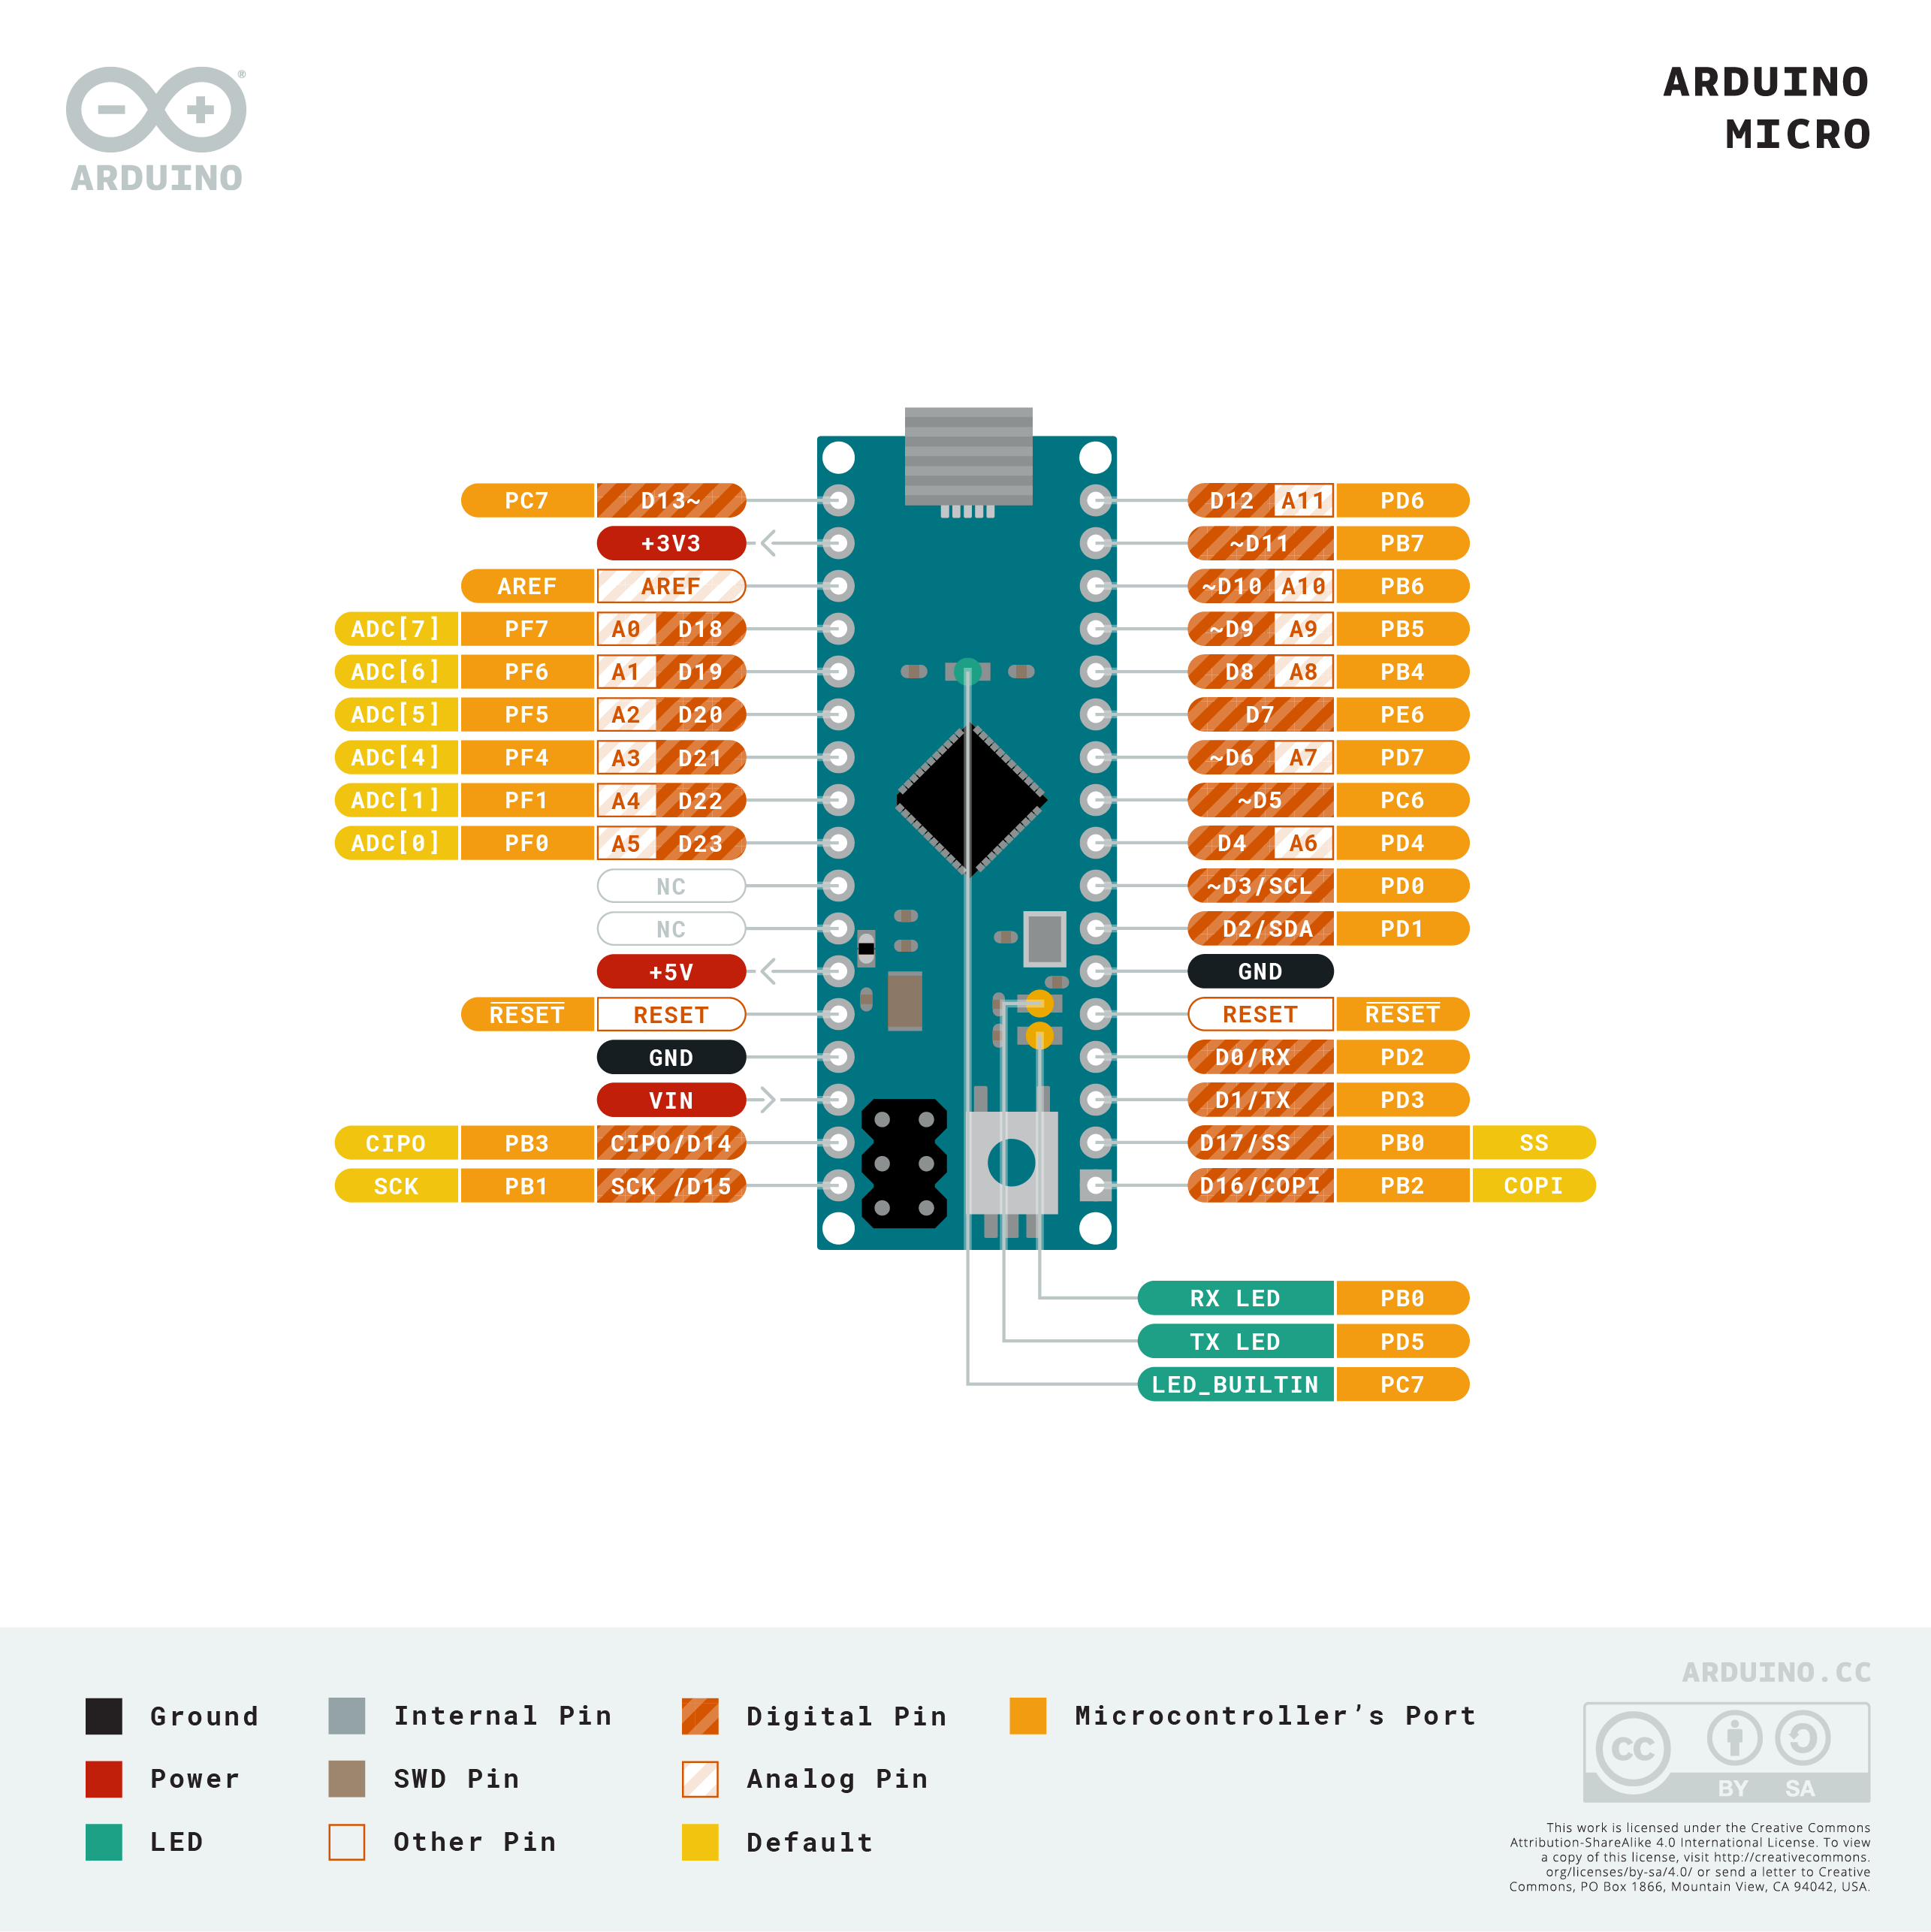
\includegraphics[width=\textwidth]{graphics/appendix/arduino_pinout.png}

%%%%%%%%%%%%%%%%%%%%%%%

\chapter{\Acf{bom}}

The following table states all components used in this workshop. It assumed that soldering stations and supplies are provided.

\begin{center}
\begin{tabular}{lllcr}
\hline
\textbf{Component}  &   \textbf{Supplier}   &   \textbf{Article \#} &   \textbf{Amount} &   \textbf{Cost total} \\
\hline\hline
Arduino Micro       &   \href{https://www.digikey.com/en/products/detail/arduino/A000053/4486332}{Digikey}             &   A000053             &   1   &   \$20.70 \\
USB Cable           &   \href{https://www.digikey.com/en/products/detail/cui-devices/CBL-UA-MUB-1/9838595?s=N4IgTCBcDaIIwAYwFoCsBOALAZmQOQBEQBdAXyA}{Digikey}             &   102-5943-ND         &   1   &   \$2.55 \\
Breadboard          &   \href{https://www.adafruit.com/product/239}{Adafruit}   &   239     &   1   &   \$5.95  \\
Breadboard wires    &   \href{https://www.adafruit.com/product/153}{Adafruit}   &   153     &   1   &   \$4.95  \\
\ac{led} red        &   \href{https://www.digikey.com/en/products/detail/broadcom-limited/HLMP-3600/637603?s=N4IgTCBcDaIKwEYBsBaBBmdBOFA5AIiALoC%2BQA}{Digikey}    &   516-1339-ND         &   1   &   \$0.81  \\
\ac{led} green      &   \href{https://www.digikey.com/en/products/detail/broadcom-limited/HLMP-3962/637598?s=N4IgTCBcDaIKwEYBsBaBBmdAWFA5AIiALoC%2BQA}{Digikey}     &   516-1334-ND &   1   &   \$0.78 \\
Buttons             &   \href{https://www.adafruit.com/product/367}{Adafruit}   &   367     &   1   &   \$2.50  \\
Resistors 1\,k$\Omega$ & \href{https://www.adafruit.com/product/4294}{Adafruit}  &   4294    &   1   &   \$0.75  \\
Resistors 10\,k$\Omega$ & \href{https://www.adafruit.com/product/2784}{Adafruit}  &   2784    &   1   &   \$0.75  \\
Display             &   \href{https://www.adafruit.com/product/1002}{Adafruit}   &   1002    &   1   &   \$10.95    \\
Thermistor          &   \href{https://www.adafruit.com/product/372}{Adafruit}   &   372     &   1   &   \$4.00  \\
\Ac{tec}            &   \href{https://www.adafruit.com/product/1335}{Adafruit}   &   1335    &   1   &   \$34.95     \\
MOSFET              &   \href{https://www.adafruit.com/product/355}{Adafruit}   &   355     &   1   &   \$1.75  \\
12\,V power supply  &   \href{https://www.adafruit.com/product/352}{Adafruit}   &   352     &   1   &   \$24.95     \\
Power jack adapter  &   \href{https://www.adafruit.com/product/368}{Adafruit}   &   368     &   1   &   \$2.00  \\
\hline
\textbf{Total cost:}    &   &   &   &   \textbf{\$118.34}   \\
\hline
\end{tabular}
\end{center}

%%%%%%%%%%%%%%%%%%%%%%%

\chapter{Open source design tools}

\section{Calculators}
\begin{itemize}
    \item \textbf{Heat sink calculator} to determine if you need a heat sink or not. \url{https://daycounter.com/Calculators/Heat-Sink-Temperature-Calculator.phtml} 
\end{itemize}

\section{Designing}
\begin{itemize}
    \item \textbf{EasyEDA}{Online designer for \acp{pcb} with large library of components and direct ordering possibilities. \url{https://easyeda.com/}}
    \item \textbf{Fritzing} Makes electronics design accessible. Easy and simple interface to draw some of your own setups, quick to get started with. Suppliers such as Adafruit have Fritzing libraries with components that you can import. \url{https://fritzing.org/}
    \item \textbf{KiCad} Cross-platform electronics design suite. \url{https://www.kicad.org/}
\end{itemize}

\section{Virtual Hardware}
\begin{itemize}
    \item \textbf{TinkerCAD} Electronic playground from Autodesk. Allows you to virtually set up electronic components and write / test code for them. \url{https://www.tinkercad.com/}
\end{itemize}

%%%%%%%%%%%%%%%%%%%%%%%

\chapter{Full wiring diagram}

\begin{figure}[h!]
    \centering
    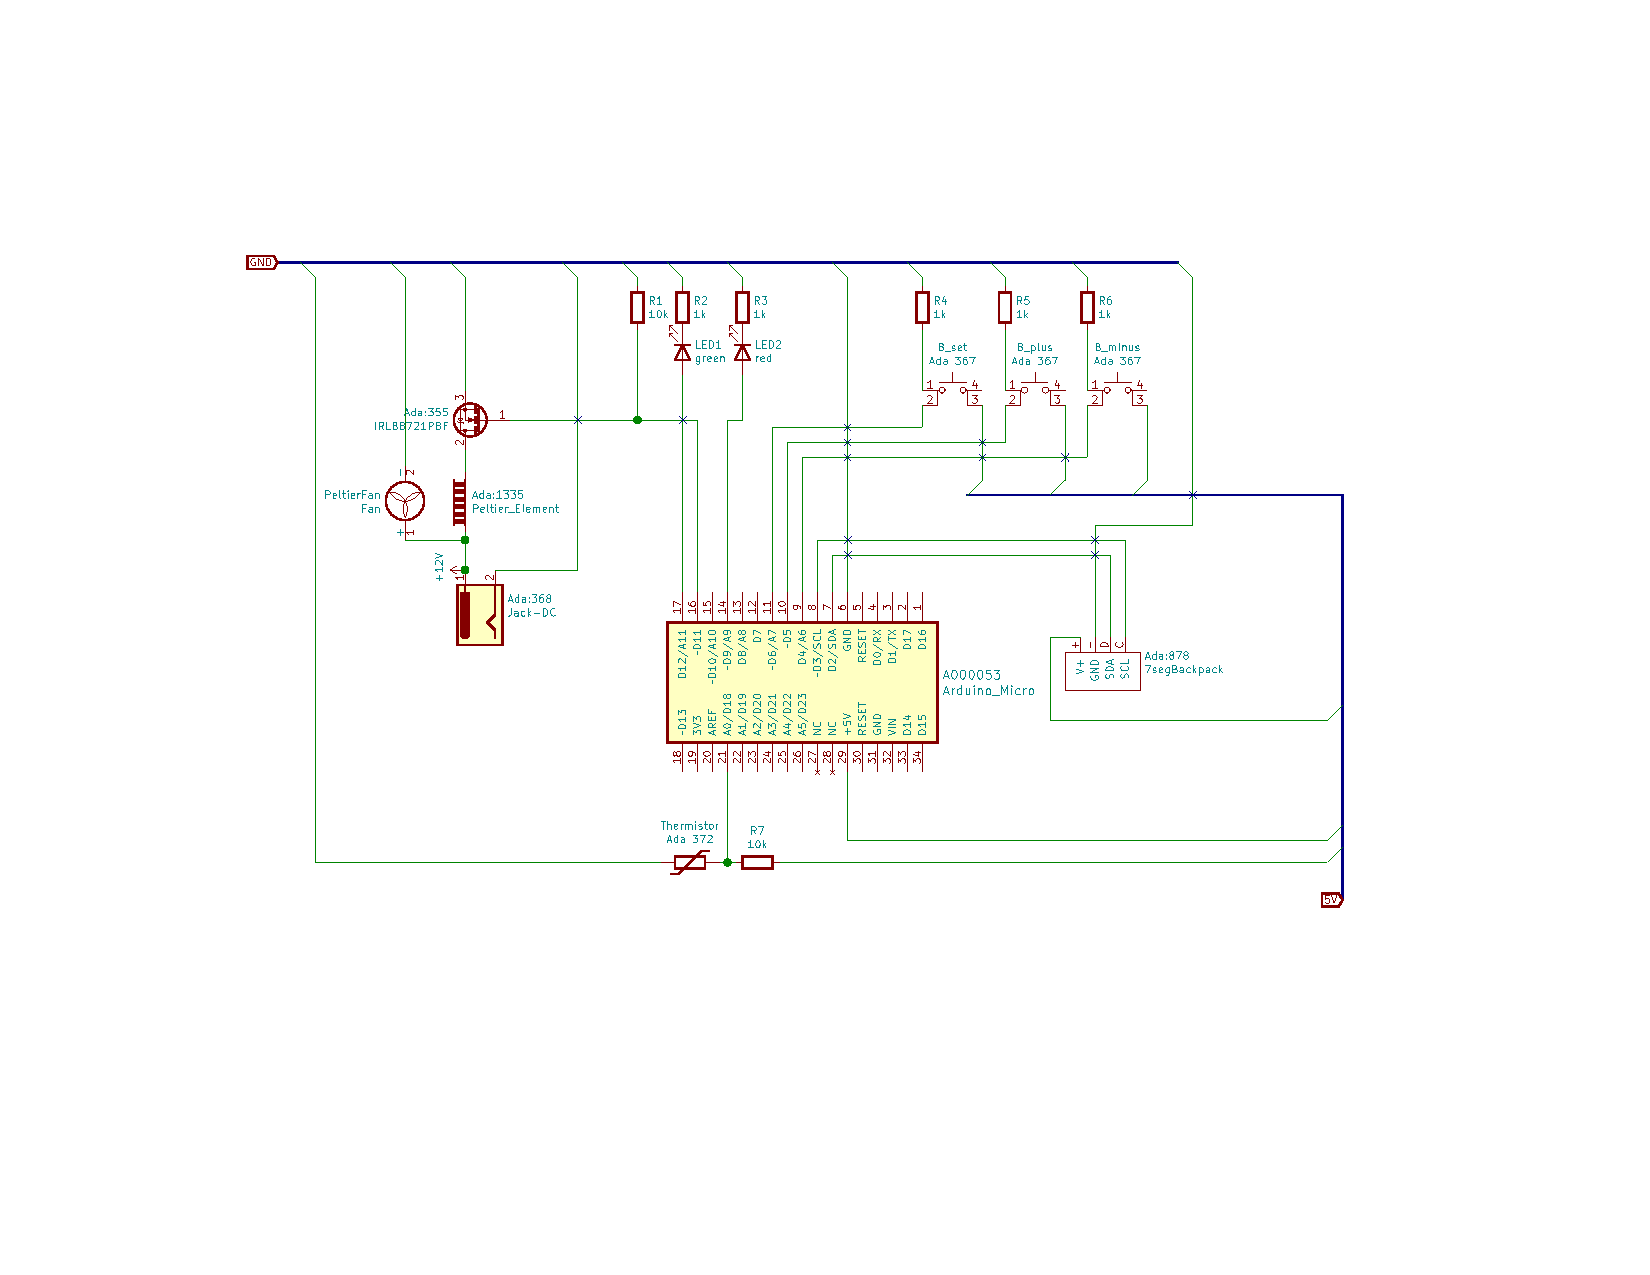
\includegraphics[width=\textwidth]{graphics/appendix/diagram_full_assembly.pdf}
    \caption{Full wiring diagram of the final project. All \href{https://www.kicad.org/}{KiCAD} files can be found on \href{https://github.com/galactic-forensics/workshop_arduino_electronics/tree/main/kicad}{GitHub}.}
    \label{fig:appendix:full_wiring_diagram}
\end{figure}


\end{document}